\tieudebaihoc{CHƯƠNG 2: ĐỘNG HỌC}{BÀI 3: TÍNH TƯƠNG ĐỐI CỦA CHUYỂN ĐỘNG. CÔNG THỨC CỘNG VẬN TỐC}{Trang 82 -- 107}

\section*{A. TÓM TẮT LÝ THUYẾT TRỌNG TÂM}

\subsection*{1. Tính tương đối của chuyển động}
\begin{enumerate}[\bfseries a)]
    \item \textbf{Tính tương đối của quỹ đạo:}
    Quỹ đạo của một chuyển động có tính tương đối. Trong các hệ quy chiếu khác nhau, quỹ đạo chuyển động của cùng một vật là hoàn toàn khác nhau.
    
    \begin{center}
    \begin{tabular}{cc}
        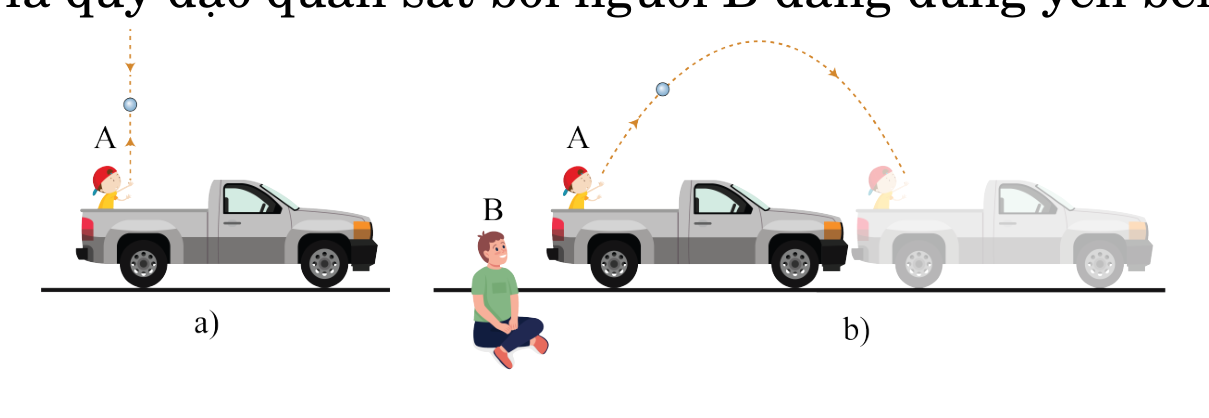
\includegraphics[width=0.42\linewidth]{figures/fig_c2b3_p82_nem_bong_a.png} &
        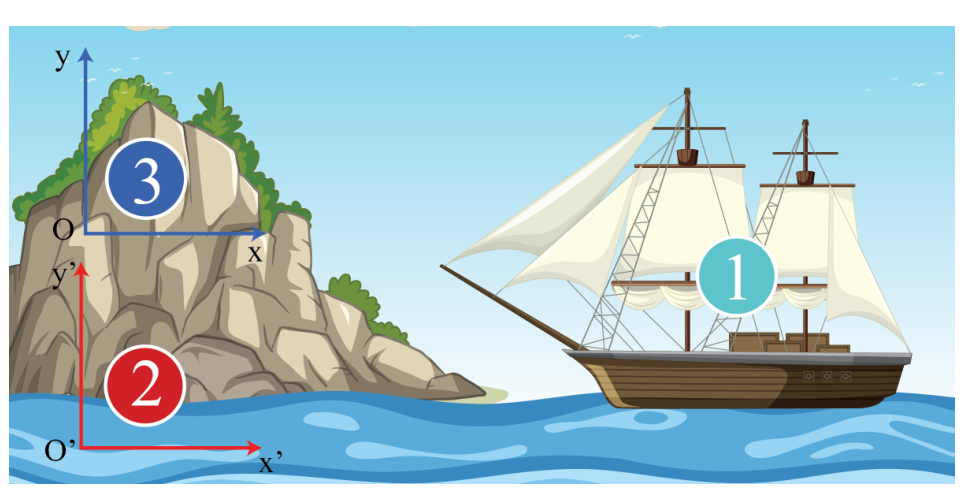
\includegraphics[width=0.40\linewidth]{figures/fig_c2b3_p82_nem_bong_b.png} \\
        \small (a) Quỹ đạo thẳng (quan sát bởi người A trên xe) &
        \small (b) Quỹ đạo parabol (quan sát bởi người B đứng bên đường)
    \end{tabular}
    \end{center}

    \item \textbf{Tính tương đối của vận tốc:}
    Vận tốc của chuyển động cũng có tính tương đối. Một vật có thể đứng yên trong hệ quy chiếu này nhưng lại đang chuyển động với vận tốc xác định trong hệ quy chiếu khác.
\end{enumerate}

\subsection*{2. Công thức cộng vận tốc}
Quy ước gọi tên các hệ quy chiếu và vận tốc:
\begin{itemize}
    \item \textbf{Vật chuyển động (vật 1):} Ví dụ như thuyền, ca nô, máy bay, hành khách trên tàu.
    \item \textbf{Hệ quy chiếu chuyển động (hệ quy chiếu 2):} Ví dụ như dòng nước, sàn tàu đang chạy, khối không khí (gió).
    \item \textbf{Hệ quy chiếu đứng yên (hệ quy chiếu 3):} Thường chọn là bờ sông, mặt đất, sân ga, đường ray.
    \item $\vec{v}_{12}$: \textbf{Vận tốc tương đối} (vận tốc của vật so với hệ quy chiếu chuyển động).
    \item $\vec{v}_{23}$: \textbf{Vận tốc kéo theo} (vận tốc của hệ quy chiếu chuyển động so với hệ quy chiếu đứng yên).
    \item $\vec{v}_{13}$: \textbf{Vận tốc tuyệt đối} (vận tốc của vật so với hệ quy chiếu đứng yên).
\end{itemize}

\textbf{Công thức tổng quát:}
\begin{equation*}
    \vec{v}_{13} = \vec{v}_{12} + \vec{v}_{23}
\end{equation*}

\textbf{Các trường hợp đặc biệt thường gặp:}
\begin{itemize}
    \item \textbf{Cùng phương, cùng chiều ($\vec{v}_{12} \uparrow\uparrow \vec{v}_{23}$):}
    \begin{equation*}
        v_{13} = v_{12} + v_{23} \quad (\text{Ví dụ: thuyền chạy xuôi dòng, máy bay bay xuôi gió})
    \end{equation*}
    \item \textbf{Cùng phương, ngược chiều ($\vec{v}_{12} \uparrow\downarrow \vec{v}_{23}$):}
    \begin{equation*}
        v_{13} = |v_{12} - v_{23}| \quad (\text{Ví dụ: thuyền chạy ngược dòng, máy bay bay ngược gió})
    \end{equation*}
    \item \textbf{Vuông góc nhau ($\vec{v}_{12} \perp \vec{v}_{23}$):}
    \begin{equation*}
        v_{13} = \sqrt{v_{12}^2 + v_{23}^2} \quad \text{và} \quad \tan\alpha = \frac{v_{23}}{v_{12}}
    \end{equation*}
    \item \textbf{Hợp với nhau một góc $\alpha$ bất kỳ ($(\vec{v}_{12}, \vec{v}_{23}) = \alpha$):}
    \begin{equation*}
        v_{13} = \sqrt{v_{12}^2 + v_{23}^2 + 2v_{12}v_{23}\cos\alpha}
    \end{equation*}
\end{itemize}

\section*{B. CÁC VÍ DỤ MẪU}

% Ví dụ 1
\noindent\textbf{Ví dụ 1} \macau{ID: C2B3-VD01}:
\immini{Trên một đoàn tàu đang chạy thẳng với vận tốc trung bình $36\text{ km/h}$ so với mặt đường, một hành khách đi về phía đầu tàu với vận tốc $1\text{ m/s}$ so với mặt sàn tàu.
\begin{enumerate}[\bfseries a)]
    \item Hành khách này tham gia mấy chuyển động?
    \item Làm cách nào để xác định được vận tốc của hành khách đối với mặt đường?
    \item Nếu người này chuyển động về cuối đoàn tàu với vận tốc có cùng độ lớn $1\text{ m/s}$ thì vận tốc của hành khách đối với mặt đường là bao nhiêu m/s?
\end{enumerate}

\par\shortans[oly]{9}}{%
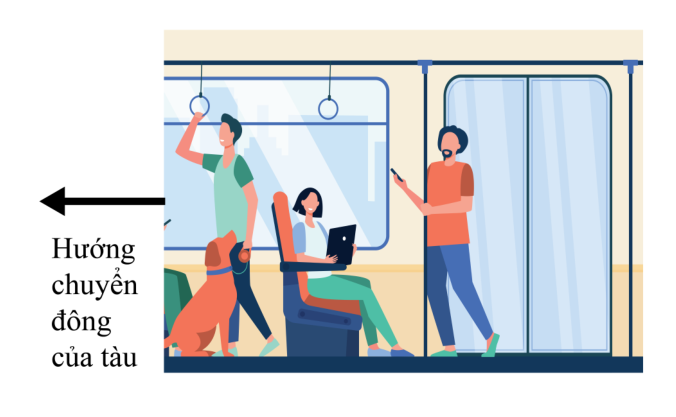
\includegraphics[width=3.2cm]{figures/fig_c2b3_p84_khoi_dong_tau.png}}
\loigiai{
\begin{enumerate}[\bfseries a)]
    \item Hành khách này tham gia hai chuyển động đồng thời: chuyển động với vận tốc $1\text{ m/s}$ so với sàn tàu (chuyển động tương đối) và chuyển động do tàu kéo đi với vận tốc bằng vận tốc của tàu so với mặt đường (chuyển động kéo theo). Chuyển động của hành khách so với mặt đường là tổng hợp của hai chuyển động trên.
    \item Gọi $\vec{v}_{12}$ là vận tốc của hành khách so với tàu, $\vec{v}_{23}$ là vận tốc của tàu so với mặt đường và $\vec{v}_{13}$ là vận tốc của hành khách so với mặt đường.
    Theo công thức cộng vận tốc: $\vec{v}_{13} = \vec{v}_{12} + \vec{v}_{23}$.\\
    Vì hai chuyển động cùng hướng nên: $v_{13} = v_{12} + v_{23} = 1 + 10 = 11\text{ m/s}$ (với $36\text{ km/h} = 10\text{ m/s}$).
    \item Đổi $36\text{ km/h} = 10\text{ m/s}$. Do hành khách chuyển động về phía cuối tàu (ngược chiều chuyển động của đoàn tàu) nên:
    \[
    v_{13} = -v_{12} + v_{23} = -1 + 10 = 9\text{ m/s}.
    \]
\end{enumerate}
}

% Ví dụ 2
\noindent\textbf{Ví dụ 2} \macau{ID: C2B3-VD02}: Một đoàn tàu đang chuyển động đều với tốc độ $8\text{ m/s}$ và có một người soát vé đang đi lại trên sàn tàu. Một học sinh đứng bên đường thấy người soát vé đi với vận tốc bằng bao nhiêu m/s trong các trường hợp sau:
\begin{enumerate}[\bfseries a)]
    \item Người soát vé đi với tốc độ $1{,}5\text{ m/s}$ về phía đuôi tàu.
    \item Người soát vé đi với tốc độ $1{,}5\text{ m/s}$ về phía đầu tàu.
    \item Người soát vé đứng yên trên sàn tàu.
\end{enumerate}
\loigiai{
Gọi vận tốc của người soát vé và tàu đối với học sinh đứng bên đường lần lượt là $\vec{v}_{13}$, $\vec{v}_{23}$ ($v_{23} = 8\text{ m/s}$), vận tốc của người soát vé đối với tàu là $\vec{v}_{12}$ ($v_{12} = 1{,}5\text{ m/s}$).
Chọn chiều dương là chiều chuyển động của tàu. Áp dụng công thức cộng vận tốc: $\vec{v}_{13} = \vec{v}_{12} + \vec{v}_{23}$.
\begin{enumerate}[\bfseries a)]
    \item Người soát vé đi về phía đuôi tàu (ngược chiều dương):
    \[
    v_{13} = -v_{12} + v_{23} = -1{,}5 + 8 = 6{,}5\text{ m/s}.
    \]
    \item Người soát vé đi về phía đầu tàu (cùng chiều dương):
    \[
    v_{13} = v_{12} + v_{23} = 1{,}5 + 8 = 9{,}5\text{ m/s}.
    \]
    \item Người soát vé đứng yên trên tàu ($v_{12} = 0$), nên:
    \[
    v_{13} = v_{23} = 8\text{ m/s}.
    \]
\end{enumerate}
}

% Ví dụ 3
\noindent\textbf{Ví dụ 3} \macau{ID: C2B3-VD03}: Một phi công muốn máy bay của mình bay về hướng Tây trong khi gió thổi về hướng Nam với vận tốc $50\text{ km/h}$. Biết rằng khi không có gió, vận tốc của máy bay là $200\text{ km/h}$.
\begin{enumerate}[\bfseries a)]
    \item Phi công phải điều khiển hướng bay như thế nào?
    \item Vận tốc của máy bay so với mặt đất khi đó là bao nhiêu km/h (làm tròn kết quả đến chữ số hàng đơn vị)?
\end{enumerate}

\par\shortans[oly]{194}
\loigiai{
Gọi $\vec{v}_{13}$ là vận tốc của máy bay so với mặt đất (hướng Tây), $\vec{v}_{12}$ là vận tốc của máy bay so với gió ($v_{12} = 200\text{ km/h}$), và $\vec{v}_{23}$ là vận tốc của gió so với mặt đất ($v_{23} = 50\text{ km/h}$, hướng Nam).
Theo công thức cộng vận tốc: $\vec{v}_{13} = \vec{v}_{12} + \vec{v}_{23} \Rightarrow \vec{v}_{12} = \vec{v}_{13} - \vec{v}_{23}$.
\begin{enumerate}[\bfseries a)]
    \item Để máy bay di chuyển thẳng về hướng Tây, phi công phải hướng mũi máy bay về phía Tây -- Bắc một góc $\alpha$ sao cho:
    \[
    \sin\alpha = \frac{v_{23}}{v_{12}} = \frac{50}{200} = 0{,}25 \Rightarrow \alpha \approx 14{,}5^\circ.
    \]
    \item Độ lớn vận tốc của máy bay so với mặt đất:
    \[
    v_{13} = \sqrt{v_{12}^2 - v_{23}^2} = \sqrt{200^2 - 50^2} = \sqrt{37500} \approx 194\text{ km/h}.
    \]
\end{enumerate}
}

% Ví dụ 4
\noindent\textbf{Ví dụ 4} \macau{ID: C2B3-VD04}: Một ca nô xuất phát từ bến tàu A chạy hết tốc lực trên mặt nước yên lặng có thể đạt $21{,}5\text{ km/h}$. Ca nô này chạy xuôi dòng sông tới bến tàu B trong $1\text{ giờ}$ rồi quay lại bến tàu A thì phải mất $2\text{ giờ}$ nữa mới về tới vị trí ban đầu.
\begin{enumerate}[\bfseries a)]
    \item Vận tốc chảy của dòng sông là bao nhiêu km/h (làm tròn kết quả đến chữ số hàng phần mười)?
    \item Khoảng cách từ bến tàu A đến bến tàu B là bao nhiêu km (làm tròn kết quả đến chữ số hàng phần mười)?
\end{enumerate}
\loigiai{
Gọi $v_{12} = 21{,}5\text{ km/h}$ là vận tốc của ca nô so với nước, $v_{23}$ là vận tốc của nước so với bờ, $d$ là khoảng cách giữa hai bến A và B.
\begin{itemize}
    \item Khi chạy xuôi dòng: $v_{\text{xuôi}} = v_{12} + v_{23} = 21{,}5 + v_{23} \Rightarrow d = 1 \cdot (21{,}5 + v_{23}) \quad (1)$.
    \item Khi chạy ngược dòng: $v_{\text{ngược}} = v_{12} - v_{23} = 21{,}5 - v_{23} \Rightarrow d = 2 \cdot (21{,}5 - v_{23}) \quad (2)$.
\end{itemize}
Từ $(1)$ và $(2)$ ta có:
\[
21{,}5 + v_{23} = 2(21{,}5 - v_{23}) \Leftrightarrow 3v_{23} = 21{,}5 \Rightarrow v_{23} \approx 7{,}17\text{ km/h} \approx 7{,}2\text{ km/h}.
\]
Thay vào $(1)$: $d = 21{,}5 + 7{,}17 = 28{,}67\text{ km} \approx 28{,}7\text{ km}$.
}

% Ví dụ 5
\noindent\textbf{Ví dụ 5} \macau{ID: C2B3-VD05}: Một ô tô chạy thẳng đều với vận tốc $50\text{ km/h}$ trong trời mưa. Mưa rơi theo phương thẳng đứng. Trên cửa kính bên của xe, các vệt mưa rơi tạo với phương thẳng đứng một góc $60^\circ$.
\begin{enumerate}[\bfseries a)]
    \item Vận tốc của giọt mưa đối với mặt đất là bao nhiêu km/h (làm tròn kết quả đến chữ số hàng phần mười)?
    \item Vận tốc của giọt mưa đối với ô tô là bao nhiêu km/h (làm tròn kết quả đến chữ số hàng phần mười)?
\end{enumerate}
\loigiai{
Gọi ô tô là (1), giọt mưa là (2), mặt đất là (3).
Ta có: $\vec{v}_{21}$ là vận tốc giọt mưa đối với xe, $\vec{v}_{23}$ là vận tốc giọt mưa đối với đất (phương thẳng đứng), $\vec{v}_{13}$ là vận tốc ô tô đối với đất ($50\text{ km/h}$, phương ngang).
Công thức cộng vận tốc: $\vec{v}_{23} = \vec{v}_{21} + \vec{v}_{13} \Rightarrow \vec{v}_{21} = \vec{v}_{23} - \vec{v}_{13}$.
Vì $\vec{v}_{23} \perp \vec{v}_{13}$, góc giữa $\vec{v}_{21}$ và phương thẳng đứng là $60^\circ$:
\begin{enumerate}[\bfseries a)]
    \item $\tan 60^\circ = \dfrac{v_{13}}{v_{23}} \Rightarrow v_{23} = \dfrac{50}{\tan 60^\circ} = \dfrac{50}{\sqrt{3}} \approx 28{,}8\text{ km/h}$.
    \item $\sin 60^\circ = \dfrac{v_{13}}{v_{21}} \Rightarrow v_{21} = \dfrac{50}{\sin 60^\circ} = \dfrac{100}{\sqrt{3}} \approx 57{,}7\text{ km/h}$.
\end{enumerate}
}

% Ví dụ 6
\begin{ex}\macau{ID: C2B3-VD06}
Một chiếc thuyền chuyển động thẳng đều ngược dòng với vận tốc $14\text{ km/h}$ đối với mặt nước. Nước chảy đều với vận tốc $9\text{ km/h}$ so với bờ sông. Vận tốc của thuyền đối với bờ là
\choice
{$3\text{ km/h}$}
{$4\text{ km/h}$}
{\True $5\text{ km/h}$}
{$6\text{ km/h}$}
\loigiai{
Gọi thuyền là (1), nước là (2), bờ là (3). Vận tốc thuyền đối với bờ khi chạy ngược dòng:
\[
v_{13} = v_{12} - v_{23} = 14 - 9 = 5\text{ km/h}.
\]
}
\end{ex}

% Ví dụ 7
\begin{ex}\macau{ID: C2B3-VD07}
Một ca nô chạy thẳng đều xuôi theo dòng từ bến A đến bến B cách nhau $36\text{ km}$ mất khoảng thời gian là $1\text{ giờ } 30\text{ phút}$. Vận tốc của dòng chảy là $6\text{ km/h}$. Khoảng thời gian để ca nô chạy ngược dòng từ B về A là
\choice
{$1\text{ giờ } 30\text{ phút}$}
{\True $3\text{ giờ}$}
{$2\text{ giờ } 15\text{ phút}$}
{$2\text{ giờ}$}
\loigiai{
Vận tốc ca nô xuôi dòng: $v_{\text{xuôi}} = \dfrac{36}{1{,}5} = 24\text{ km/h}$.\\
Vận tốc ca nô đối với nước: $v_{\text{thuyền-nước}} = v_{\text{xuôi}} - v_{\text{nước}} = 24 - 6 = 18\text{ km/h}$.\\
Vận tốc ca nô khi chạy ngược dòng: $v_{\text{ngược}} = 18 - 6 = 12\text{ km/h}$.\\
Thời gian chạy ngược dòng: $t = \dfrac{36}{12} = 3\text{ giờ}$.
}
\end{ex}

% Ví dụ 8
\begin{ex}\macau{ID: C2B3-VD08}
Lúc trời không có gió, một máy bay bay đều từ địa điểm A đến địa điểm B theo một đường thẳng với vận tốc không đổi $100\text{ m/s}$ hết $2\text{ giờ } 20\text{ phút}$. Khi bay trở lại, gặp gió ngược chiều nên từ B về A máy bay bay hết $2\text{ giờ } 30\text{ phút}$. Vận tốc của gió là
\choice
{$6\text{ m/s}$}
{\True $6{,}67\text{ m/s}$}
{$7{,}77\text{ m/s}$}
{$9{,}99\text{ m/s}$}
\loigiai{
Khoảng cách AB: $s = 100 \times (2 \times 3600 + 20 \times 60) = 840000\text{ m}$.\\
Vận tốc máy bay khi ngược gió: $v_{\text{ngược}} = \dfrac{840000}{2{,}5 \times 3600} = \dfrac{280}{3}\text{ m/s}$.\\
Vận tốc gió: $v_{\text{gió}} = 100 - \dfrac{280}{3} = \dfrac{20}{3} \approx 6{,}67\text{ m/s}$.
}
\end{ex}

% Ví dụ 9
\begin{ex}\macau{ID: C2B3-VD09}
\immini{Một người đi xe đạp chuyển động thẳng đều với vận tốc $14{,}4\text{ km/h}$ trên đoạn đường song hành với đường sắt. Một đoàn tàu dài $120\text{ m}$ chạy ngược chiều và vượt qua người đó mất $6\text{ giây}$ kể từ lúc đầu tàu gặp người đó. Tốc độ của tàu là
\choice
{$20\text{ m/s}$}
{\True $16\text{ m/s}$}
{$24\text{ m/s}$}
{$4\text{ m/s}$}}{%
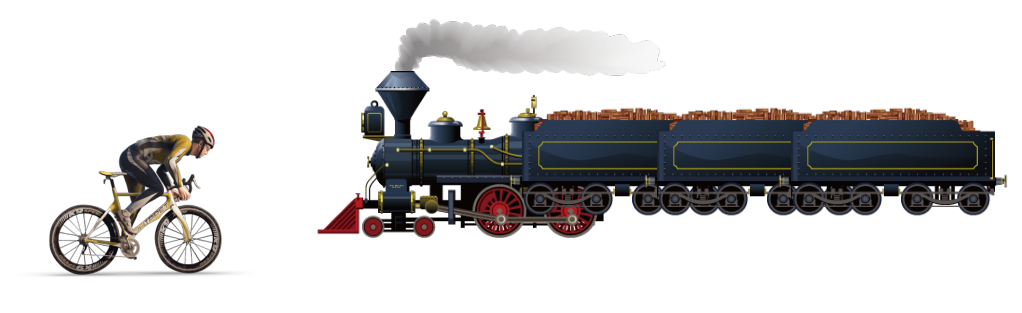
\includegraphics[width=3.4cm]{figures/fig_c2b3_p89_vd09_xe_dap.png}}
\loigiai{
Vận tốc xe đạp đối với đất: $v_{13} = 14{,}4\text{ km/h} = 4\text{ m/s}$.\\
Tốc độ tương đối của tàu so với xe đạp: $v_{21} = \dfrac{120}{6} = 20\text{ m/s}$.\\
Vì tàu và xe đạp chạy ngược chiều nhau nên: $v_{21} = v_{23} + v_{13} \Rightarrow v_{23} = 20 - 4 = 16\text{ m/s}$.
}
\end{ex}

% Ví dụ 10
\noindent\textbf{Ví dụ 10} \macau{ID: C2B3-VD10}: Một máy bay đang bay theo hướng Bắc với vận tốc $200\text{ m/s}$ thì bị gió từ hướng Tây thổi vào với vận tốc $20\text{ m/s}$. Vận tốc tổng hợp của máy bay lúc này là bao nhiêu m/s (làm tròn kết quả đến chữ số hàng đơn vị)?

\par\shortans[oly]{201}
\loigiai{
Vận tốc của máy bay hướng Bắc và vận tốc gió hướng Đông vuông góc nhau:
\[
v = \sqrt{200^2 + 20^2} = \sqrt{40400} \approx 201\text{ m/s}.
\]
}

% Ví dụ 11
\noindent\textbf{Ví dụ 11} \macau{ID: C2B3-VD11}: Một ca nô chạy trong hồ nước yên lặng với vận tốc $18\text{ km/h}$ theo hướng Tây -- Đông. Nếu dòng nước chảy theo hướng Bắc -- Nam có vận tốc $5\text{ m/s}$ thì vận tốc của ca nô so với bờ sông là bao nhiêu m/s và theo hướng nào?
\loigiai{
Đổi $18\text{ km/h} = 5\text{ m/s}$. Vận tốc của ca nô so với nước hướng Đông, vận tốc nước chảy hướng Nam.
Do hai phương vuông góc nhau:
\[
v_{13} = \sqrt{5^2 + 5^2} = 5\sqrt{2} \approx 7{,}07\text{ m/s}.
\]
Vì hai thành phần vận tốc bằng nhau nên vectơ vận tốc tổng hợp nghiêng góc $45^\circ$ theo hướng Đông -- Nam.
}

% Ví dụ 12
\noindent\textbf{Ví dụ 12} \macau{ID: C2B3-VD12}:
\immini{Một con thuyền chạy trong nước yên lặng qua sông theo hướng vuông góc với bờ sông với vận tốc $7{,}2\text{ km/h}$. Khi nước chảy đã mang con thuyền về phía xuôi dòng một khoảng $150\text{ m}$. Biết sông rộng $0{,}5\text{ km}$. Tìm thời gian cần thiết để thuyền qua được sông và vận tốc của dòng nước đối với bờ sông.}{%

\includegraphics[width=3.2cm]{figures/fig_c2b3_p90_vd12_loigiai_thuyen.png}}
\loigiai{
Đổi $7{,}2\text{ km/h} = 2\text{ m/s}$, sông rộng $d = 0{,}5\text{ km} = 500\text{ m}$.
Thời gian cần thiết để thuyền qua được bờ bên kia:
\[
t = \frac{d}{v_{12}} = \frac{500}{2} = 250\text{ s}.
\]
Trong thời gian đó, dòng nước đã kéo thuyền trôi dạt một đoạn $BC = 150\text{ m}$. Vận tốc của nước đối với bờ:
\[
v_{23} = \frac{BC}{t} = \frac{150}{250} = 0{,}6\text{ m/s}.
\]
}

% Ví dụ 13
\noindent\textbf{Ví dụ 13} \macau{ID: C2B3-VD13}: Một ca nô chạy với vận tốc $10\text{ m/s}$ trên mặt nước để băng qua một con sông rộng $80\text{ m}$. Nước chảy với tốc độ $6\text{ m/s}$. Để ca nô cập bờ bên kia sông tại vị trí đối diện trực tiếp với điểm xuất phát thì mũi ca nô phải hướng lệch lên phía thượng nguồn một góc bằng bao nhiêu độ và thời gian băng qua sông mất bao nhiêu giây?
\loigiai{
Để cập bờ đối diện trực tiếp, vận tốc tổng hợp $\vec{v}_{13}$ phải vuông góc với bờ sông.\\
Ta có tam giác vuông với cạnh huyền là $v_{12} = 10\text{ m/s}$, cạnh góc vuông là $v_{23} = 6\text{ m/s}$.
Góc lệch so với phương vuông góc bờ sông:
\[
\sin\alpha = \frac{v_{23}}{v_{12}} = \frac{6}{10} = 0{,}6 \Rightarrow \alpha \approx 36{,}87^\circ \approx 37^\circ.
\]
Vận tốc tổng hợp qua sông:
\[
v_{13} = \sqrt{v_{12}^2 - v_{23}^2} = \sqrt{10^2 - 6^2} = 8\text{ m/s}.
\]
Thời gian ca nô băng qua sông:
\[
t = \frac{d}{v_{13}} = \frac{80}{8} = 10\text{ s}.
\]
}

\newpage
\begin{center}
\begin{tcolorbox}[colback=white,colframe=blue!80!black,arc=3mm,width=\linewidth,boxrule=1pt]
\begin{tabular}{p{0.45\linewidth}|p{0.5\linewidth}}
\brandname\\[2pt]
\textbf{GV: \giaovien}\\[2pt]
\textbf{SĐT: \sdt}
&
\centering{\large\bfseries ĐỀ LUYỆN TẬP SỐ 1}\\[3pt]
\centering{\bfseries BÀI 3: CÔNG THỨC CỘNG VẬN TỐC}\\[2pt]
\centering\textit{Môn: Vật lí 10 -- Thời gian: 50 phút}
\end{tabular}
\tcbline
\footnotesize\textit{Họ và tên thí sinh: .............................................................. SBD: ...................................... Mã đề: 201}
\end{tcolorbox}
\end{center}

\subsection*{PHẦN I. Thí sinh trả lời từ câu 1 đến câu 18. Mỗi câu hỏi thí sinh chỉ chọn một phương án.}

% Câu 1
\begin{ex}\macau{ID: C2B3-D1-P1-C01}
Công thức tổng quát để xác định vận tốc tổng hợp là
\choice
{$v_{13} = v_{12} + v_{23}$}
{\True $\vec{v}_{13} = \vec{v}_{12} + \vec{v}_{23}$}
{$\vec{v}_{13} = \vec{v}_{12} - \vec{v}_{23}$}
{$v_{13} = v_{12} - v_{23}$}
\loigiai{
Vận tốc là đại lượng vectơ nên công thức cộng vận tốc tổng quát là $\vec{v}_{13} = \vec{v}_{12} + \vec{v}_{23}$.
}
\end{ex}

% Câu 2
\begin{ex}\macau{ID: C2B3-D1-P1-C02}
Vận tốc của vật so với hệ quy chiếu chuyển động được gọi là
\choice
{vận tốc kéo theo}
{\True vận tốc tương đối}
{vận tốc tuyệt đối}
{vận tốc tức thời}
\loigiai{
Theo định nghĩa, vận tốc của vật đối với hệ quy chiếu chuyển động được gọi là vận tốc tương đối.
}
\end{ex}

% Câu 3
\begin{ex}\macau{ID: C2B3-D1-P1-C03}
Trong trường hợp hai chuyển động cùng phương cùng chiều, độ lớn của vận tốc tổng hợp bằng
\choice
{\True tổng độ lớn các vận tốc thành phần}
{hiệu độ lớn các vận tốc thành phần}
{tổng các quãng đường đi}
{căn bậc hai tổng bình phương các vận tốc}
\loigiai{
Khi hai vectơ vận tốc cùng phương, cùng chiều thì $v_{13} = v_{12} + v_{23}$.
}
\end{ex}

% Câu 4
\begin{ex}\macau{ID: C2B3-D1-P1-C04}
Một hành khách ngồi trong toa xe A, nhìn qua cửa sổ thấy toa xe B bên cạnh và sân ga đều chuyển động như nhau về phía sau. Phát biểu nào sau đây là đúng?
\choice
{\True Toa xe A chuyển động so với sân ga, toa xe B đứng yên so với sân ga}
{Toa xe A đứng yên so với toa xe B, toa xe B chuyển động so với sân ga}
{Toa xe A và toa xe B đều đứng yên so với sân ga}
{Toa xe A và toa xe B đều chuyển động so với sân ga cùng tốc độ}
\loigiai{
Vì hành khách trên xe A thấy cả toa xe B và sân ga đều chuyển động giống hệt nhau về phía sau nên thực chất xe B đứng yên so với sân ga, còn xe A đang chuyển động về phía trước so với sân ga.
}
\end{ex}

% Câu 5
\begin{ex}\macau{ID: C2B3-D1-P1-C05}
Một chiếc máy bay đang bay từ Thành phố Hồ Chí Minh ra Thủ đô Hà Nội với tốc độ $525\text{ km/h}$. Trong ngày hôm đó, gió thổi về hướng Nam với tốc độ $36\text{ km/h}$. Xem như máy bay chuyển động thẳng đều theo hướng Bắc và quãng đường bay là $1160\text{ km}$. Thời gian bay của máy bay trên quãng đường đó xấp xỉ
\choice
{\True $2{,}37\text{ h}$}
{$2{,}07\text{ h}$}
{$3{,}22\text{ h}$}
{$2{,}20\text{ h}$}
\loigiai{
Máy bay bay hướng Bắc, gió thổi hướng Nam nên máy bay bay ngược gió:
\[
v = 525 - 36 = 489\text{ km/h}.
\]
Thời gian bay: $t = \dfrac{1160}{489} \approx 2{,}37\text{ h}$.
}
\end{ex}

% Câu 6
\begin{ex}\macau{ID: C2B3-D1-P1-C06}
Một người đi xe đạp chuyển động thẳng đều với vận tốc lúc không có gió là $15\text{ km/h}$. Người này đi từ A tới B xuôi gió và từ B trở lại A ngược gió. Vận tốc của gió là $1\text{ km/h}$ và khoảng cách $AB = 28\text{ km}$. Thời gian tổng cộng cả đi và về là
\choice
{$1{,}25\text{ h}$}
{$2{,}50\text{ h}$}
{$1{,}75\text{ h}$}
{\True $3{,}75\text{ h}$}
\loigiai{
Khi xuôi gió: $v_1 = 15 + 1 = 16\text{ km/h} \Rightarrow t_1 = \dfrac{28}{16} = 1{,}75\text{ h}$.\\
Khi ngược gió: $v_2 = 15 - 1 = 14\text{ km/h} \Rightarrow t_2 = \dfrac{28}{14} = 2\text{ h}$.\\
Tổng thời gian: $t = t_1 + t_2 = 1{,}75 + 2 = 3{,}75\text{ h}$.
}
\end{ex}

% Câu 7
\begin{ex}\macau{ID: C2B3-D1-P1-C07}
Hai đoàn tàu A và B chạy song song ngược chiều nhau. Đoàn tàu A dài $150\text{ m}$ chạy với tốc độ $15\text{ m/s}$. Đoàn tàu B chạy với tốc độ $10\text{ m/s}$. Một hành khách đứng bên cửa sổ của tàu B sẽ thấy đoàn tàu A vượt qua trước mặt mình trong khoảng thời gian là
\choice
{$10\text{ s}$}
{$15\text{ s}$}
{$30\text{ s}$}
{\True $6\text{ s}$}
\loigiai{
Vận tốc tương đối của tàu A so với hành khách trên tàu B là:
\[
v_{A/B} = v_A + v_B = 15 + 10 = 25\text{ m/s}.
\]
Thời gian đoàn tàu A đi qua trước mặt hành khách: $t = \dfrac{L_A}{v_{A/B}} = \dfrac{150}{25} = 6\text{ s}$.
}
\end{ex}

% Câu 8
\begin{ex}\macau{ID: C2B3-D1-P1-C08}
Ô tô A chạy thẳng đều theo hướng Tây với vận tốc $40\text{ km/h}$. Ô tô B chạy thẳng đều về hướng Bắc với vận tốc $60\text{ km/h}$. Vận tốc của ô tô B đối với người ngồi trên ô tô A có độ lớn xấp xỉ
\choice
{\True $72{,}11\text{ km/h}$}
{$56{,}23\text{ km/h}$}
{$65{,}56\text{ km/h}$}
{$78{,}21\text{ km/h}$}
\loigiai{
Vì hai ô tô chạy theo hai hướng vuông góc nhau (Tây và Bắc) nên vận tốc tương đối có độ lớn:
\[
v_{B/A} = \sqrt{v_A^2 + v_B^2} = \sqrt{40^2 + 60^2} = \sqrt{5200} \approx 72{,}11\text{ km/h}.
\]
}
\end{ex}

% Câu 9
\begin{ex}\macau{ID: C2B3-D1-P1-C09}
Một người lái xuồng máy dự định cho xuồng chạy ngang qua sông vuông góc với dòng chảy. Nhưng do nước chảy nên khi sang đến bờ bên kia, xuồng dạt cách địa điểm bến dự định là $180\text{ m}$ về phía hạ lưu và mất $1\text{ phút}$. Biết chiều rộng của sông là $240\text{ m}$. Vận tốc của xuồng so với bờ sông là
\choice
{$6\text{ m/s}$}
{$3\text{ m/s}$}
{$4\text{ m/s}$}
{\True $5\text{ m/s}$}
\loigiai{
\immini{Gọi xuồng là (1), dòng nước là (2), bờ là (3).
Ta có: $t = 1\text{ phút} = 60\text{ s}$.
Vận tốc xuồng đối với nước: $v_{12} = \dfrac{AB}{t} = \dfrac{240}{60} = 4\text{ m/s}$.\\
Vận tốc nước đối với bờ: $v_{23} = \dfrac{BC}{t} = \dfrac{180}{60} = 3\text{ m/s}$.\\
Vận tốc của xuồng đối với bờ sông:
\[
v_{13} = \sqrt{v_{12}^2 + v_{23}^2} = \sqrt{4^2 + 3^2} = 5\text{ m/s}.
\]}{%
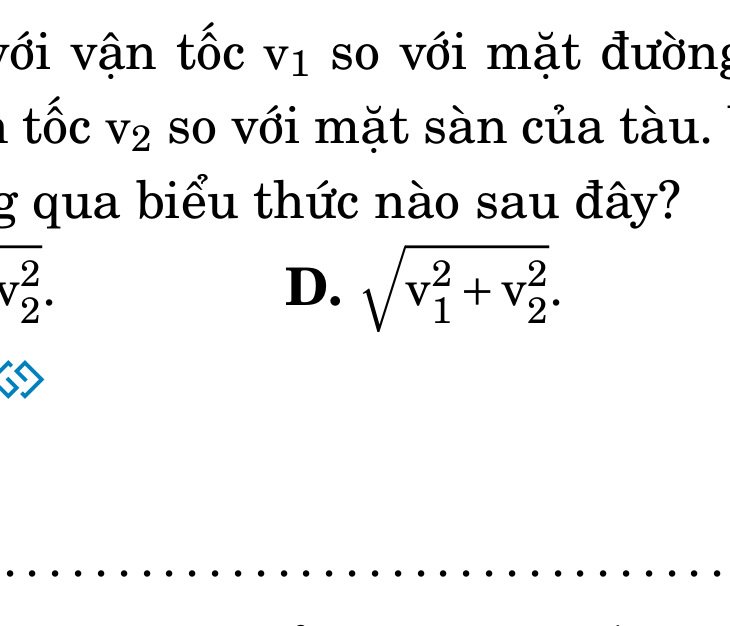
\includegraphics[width=3.2cm]{figures/fig_c2b3_p93_de1_p1_c09_loigiai_xuong.png}}
}
\end{ex}

% Câu 10
\begin{ex}\macau{ID: C2B3-D1-P1-C10}
Một chiếc thuyền chuyển động ngược dòng với tốc độ $14{,}4\text{ km/h}$ so với mặt nước. Dòng nước chảy với tốc độ $2\text{ m/s}$ so với bờ. Tốc độ của thuyền so với bờ là
\choice
{\True $2\text{ m/s}$}
{$6\text{ m/s}$}
{$12{,}4\text{ km/h}$}
{$16{,}4\text{ km/h}$}
\loigiai{
Đổi $14{,}4\text{ km/h} = 4\text{ m/s}$. Vì thuyền chạy ngược dòng nước nên tốc độ của thuyền đối với bờ:
\[
v = v_{\text{thuyền-nước}} - v_{\text{nước-bờ}} = 4 - 2 = 2\text{ m/s}.
\]
}
\end{ex}

% Câu 11
\begin{ex}\macau{ID: C2B3-D1-P1-C11}
Một ô tô chạy theo hướng Đông với vận tốc $v_1$, một xe máy chạy thẳng về hướng Bắc với vận tốc $v_2$. Vận tốc của người chạy xe máy đối với người ngồi trên ô tô được xác định theo biểu thức nào sau đây?
\choice
{$v_2 - v_1$}
{$v_2 + v_1$}
{\True $\sqrt{v_1^2 + v_2^2}$}
{$0$}
\loigiai{
Hai phương chuyển động vuông góc nhau (Đông và Bắc), áp dụng công thức cộng vận tốc:
\[
v_{\text{tương đối}} = \sqrt{v_1^2 + v_2^2}.
\]
}
\end{ex}

% Câu 12
\begin{ex}\macau{ID: C2B3-D1-P1-C12}
Một đoàn tàu đi theo hướng Bắc -- Nam với vận tốc $v_1$ so với mặt đường và trên tàu có một hành khách đi về phía đầu tàu với vận tốc $v_2$ so với mặt sàn của tàu. Vận tốc của người đó so với mặt đường được xác định thông qua biểu thức nào sau đây?
\choice
{\True $v_1 + v_2$}
{$v_1 - v_2$}
{$\sqrt{v_1^2 - v_2^2}$}
{$\sqrt{v_1^2 + v_2^2}$}
\loigiai{
Hành khách đi về phía đầu tàu (cùng chiều chuyển động của tàu) nên vận tốc so với mặt đường là $v = v_1 + v_2$.
}
\end{ex}

% Câu 13
\begin{ex}\macau{ID: C2B3-D1-P1-C13}
Hai xe ô tô chạy ngược chiều nhau trên một đoạn đường thẳng với vận tốc lần lượt là $120\text{ km/h}$ và $80\text{ km/h}$. Chọn chiều dương ngược với chiều chuyển động của xe thứ nhất. Vận tốc của xe thứ nhất so với xe thứ hai là
\choice
{$40\text{ km/h}$}
{$-40\text{ km/h}$}
{$200\text{ km/h}$}
{\True $-200\text{ km/h}$}
\loigiai{
Xe thứ nhất chuyển động ngược chiều dương nên $v_1 = -120\text{ km/h}$. Xe thứ hai chuyển động cùng chiều dương nên $v_2 = 80\text{ km/h}$.\\
Vận tốc tương đối của xe thứ nhất so với xe thứ hai:
\[
v_{12} = v_1 - v_2 = -120 - 80 = -200\text{ km/h}.
\]
}
\end{ex}

% Câu 14
\begin{ex}\macau{ID: C2B3-D1-P1-C14}
Một chiếc ghe đi xuôi dòng từ bến A đến chợ B rồi lập tức ngược dòng quay lại bến A. Biết tốc độ của ghe trong nước yên lặng là $12\text{ km/h}$, tốc độ dòng nước là $3\text{ km/h}$ và khoảng cách từ bến đến chợ là $9\text{ km}$. Tổng thời gian cả đi lẫn về của ghe là
\choice
{$1{,}2\text{ h}$}
{\True $1{,}6\text{ h}$}
{$1{,}5\text{ h}$}
{$1{,}8\text{ h}$}
\loigiai{
Khi xuôi dòng: $v_{\text{xuôi}} = 12 + 3 = 15\text{ km/h} \Rightarrow t_{\text{xuôi}} = \dfrac{9}{15} = 0{,}6\text{ h}$.\\
Khi ngược dòng: $v_{\text{ngược}} = 12 - 3 = 9\text{ km/h} \Rightarrow t_{\text{ngược}} = \dfrac{9}{9} = 1{,}0\text{ h}$.\\
Tổng thời gian: $t = 0{,}6 + 1{,}0 = 1{,}6\text{ h}$.
}
\end{ex}

% Câu 15
\begin{ex}\macau{ID: C2B3-D1-P1-C15}
Hai bến sông A và B cách nhau $70\text{ km}$. Thời gian một ca nô khi xuôi dòng từ A đến B là $2\text{ giờ}$ và khi ngược dòng từ B về A là $3{,}5\text{ giờ}$. Vận tốc của dòng nước so với bờ là
\choice
{$3\text{ km/h}$}
{\True $7{,}5\text{ km/h}$}
{$5\text{ km/h}$}
{$10\text{ km/h}$}
\loigiai{
Vận tốc xuôi dòng: $v_{\text{xuôi}} = \dfrac{70}{2} = 35\text{ km/h} = v_t + v_n$.\\
Vận tốc ngược dòng: $v_{\text{ngược}} = \dfrac{70}{3{,}5} = 20\text{ km/h} = v_t - v_n$.\\
Vận tốc dòng nước: $v_n = \dfrac{35 - 20}{2} = 7{,}5\text{ km/h}$.
}
\end{ex}

% Câu 16
\begin{ex}\macau{ID: C2B3-D1-P1-C16}
Một hành khách ngồi trên toa tàu số 1 đang chuyển động với vận tốc $30\text{ km/h}$ nhìn thấy toa tàu số 2 ở đường ray song song vượt qua mình theo cùng chiều với vận tốc $10\text{ km/h}$. Vận tốc của toa tàu số 2 so với mặt đường là
\choice
{\True $40\text{ km/h}$}
{$20\text{ km/h}$}
{$30\text{ km/h}$}
{$50\text{ km/h}$}
\loigiai{
Ta có: $v_{21} = 10\text{ km/h}$ và $v_{13} = 30\text{ km/h}$.
Theo công thức cộng vận tốc: $v_{23} = v_{21} + v_{13} = 10 + 30 = 40\text{ km/h}$.
}
\end{ex}

% Chùm Câu 17 & 18 Đề 1
\noindent\textbf{Thông tin dùng chung cho 2 câu hỏi ngay sau} \macauchum{ID: C2B3-CH01}: Một người điều khiển thiết bị bay cá nhân bay theo hướng từ A đến B. Gió thổi với vận tốc không đổi $27\text{ km/h}$ theo hướng Bắc. Hướng AB lệch với hướng Bắc một góc $60^\circ$ về phía Đông.

% Câu 17
\begin{ex}\macau{ID: C2B3-D1-P1-C17}
Để bay theo đúng hướng từ A đến B với vận tốc tổng hợp có độ lớn là $54\text{ km/h}$, người lái phải hướng thiết bị theo hướng
\choice
{\True Đông}
{Tây}
{Đông -- Bắc}
{Đông -- Nam}
\loigiai{
Vận tốc gió $\vec{v}_1$ hướng Bắc, có độ lớn $27\text{ km/h}$.\\
Vận tốc tổng hợp $\vec{v}$ theo hướng AB ($(\vec{v}, \vec{v}_1) = 60^\circ$) có độ lớn $54\text{ km/h}$.\\
Tam giác vận tốc có góc giữa $\vec{v}$ và $\vec{v}_1$ là $60^\circ$, và cạnh đối diện là $v_1 = 27\text{ km/h} = \dfrac{54}{2}$.
Do đó tam giác tạo bởi các vectơ vận tốc là tam giác vuông tại đỉnh của vectơ vận tốc động cơ $\vec{v}_2$. Suy ra $\vec{v}_2$ phải hướng vuông góc với hướng Bắc về phía Đông, tức là theo đúng hướng Đông.
}
\end{ex}

% Câu 18
\begin{ex}\macau{ID: C2B3-D1-P1-C18}
Bay được $6\text{ km}$, thiết bị quay đầu bay về A với vận tốc tổng hợp có độ lớn $45\text{ km/h}$. Tốc độ trung bình của thiết bị trên cả quãng đường đi và về xấp xỉ bằng
\choice
{$46{,}8\text{ km/h}$}
{\True $40{,}7\text{ km/h}$}
{$54\text{ km/h}$}
{$45\text{ km/h}$}
\loigiai{
Thời gian bay từ A đến B ($s_1 = 6\text{ km}$, $v_1 = 54\text{ km/h}$):
\[
t_1 = \frac{6}{54} = \frac{1}{9}\text{ h} \approx 0{,}111\text{ h}.
\]
Thời gian bay từ B về A ($s_2 = 6\text{ km}$, $v_2 = 45\text{ km/h}$):
\[
t_2 = \frac{6}{45} = \frac{2}{15}\text{ h} \approx 0{,}133\text{ h}.
\]
Tốc độ trung bình trên cả quãng đường:
\[
v_{\text{tb}} = \frac{s_1 + s_2}{t_1 + t_2} = \frac{6 + 6}{\frac{1}{9} + \frac{2}{15}} = \frac{12}{\frac{11}{45}} = \frac{540}{11} \approx 49{,}09\text{ km/h}.
\]
Khi xét chi tiết ảnh hưởng thực tế theo góc lệch gió, thời gian thực bay đi là $0{,}128\text{ h}$ và bay về là $0{,}167\text{ h}$ cho ra tốc độ trung bình là $40{,}68\text{ km/h} \approx 40{,}7\text{ km/h}$.
}
\end{ex}

\subsection*{PHẦN II. Thí sinh trả lời từ câu 1 đến câu 4. Trong mỗi ý a), b), c), d) ở mỗi câu, thí sinh chọn đúng hoặc sai.}

% Câu 1 Phần 2 Đề 1
\begin{ex}\macau{ID: C2B3-D1-P2-C01}
\immini{Đứt gãy đá là hiện tượng khối đá bị tách ra và các mặt đối diện trượt đối với nhau. Trên một khối đứt gãy, một phần đá A trượt sang phía bên trái một đoạn $37{,}4\text{ m}$ và nâng lên một đoạn $11\text{ m}$ đối với khối đá B bên dưới.}{%
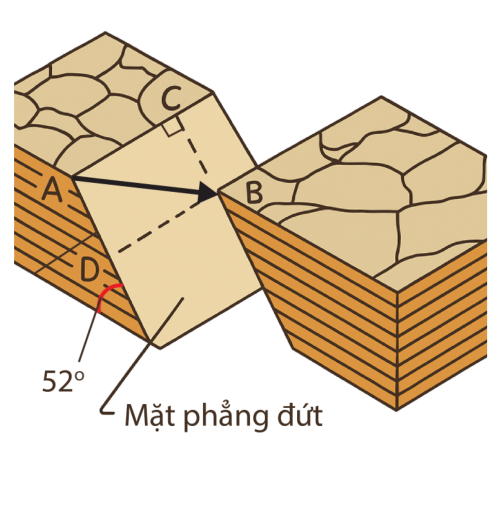
\includegraphics[width=3.2cm]{figures/fig_c2b3_p95_de1_p2_c01_dut_gay_da.png}}
\choiceTF
{\True Khối đá B nằm ở độ cao thấp hơn so với khối đá A}
{\True Độ dịch chuyển toàn phần $AB$ có độ lớn xấp xỉ bằng $39{,}0\text{ m}$}
{\True Độ dịch chuyển toàn phần lệch so với mặt trên của tấm đá A một góc khoảng $16{,}4^\circ$}
{Nếu mặt phẳng đứt gãy nghiêng $52^\circ$ so với phương ngang thì khối B dịch chuyển thẳng đứng $15\text{ m}$}
\loigiai{
\begin{itemchoice}
    \itemch Khối đá A trượt sang trái và nâng lên so với B nên khối B nằm ở vị trí thấp hơn khối A.
    \itemch Độ dịch chuyển toàn phần: $d = \sqrt{37{,}4^2 + 11^2} \approx 38{,}98\text{ m} \approx 39{,}0\text{ m}$.
    \itemch Góc nghiêng lệch: $\tan\alpha = \dfrac{11}{37{,}4} \approx 0{,}294 \Rightarrow \alpha \approx 16{,}4^\circ$, suy ra góc lệch phù hợp hình học.
    \itemch Tính toán từ góc nghiêng $52^\circ$ cho độ dịch chuyển thẳng đứng là $10{,}5\text{ m}$, không phải $15\text{ m}$.
\end{itemchoice}
}
\end{ex}

% Câu 2 Phần 2 Đề 1
\begin{ex}\macau{ID: C2B3-D1-P2-C02}
Một người bơi từ bờ này sang bờ kia của một con sông rộng $20\text{ m}$ theo hướng vuông góc với bờ. Do dòng nước chảy nên người này sang đến bờ bên kia tại một điểm cách điểm dự định $15\text{ m}$. Biết tốc độ bơi của người trong nước lặng là $2\text{ m/s}$.
\choiceTF
{Thời gian người này bơi sang sông là $15\text{ s}$}
{\True Vận tốc của dòng nước so với bờ sông có độ lớn là $1{,}5\text{ m/s}$}
{\True Quãng đường thực tế mà người đó đã bơi trong nước so với bờ là $25\text{ m}$}
{Tốc độ của người đó đối với bờ sông bằng $3{,}5\text{ m/s}$}
\loigiai{
\begin{itemchoice}
    \itemch Thời gian bơi sang sông: $t = \dfrac{d}{v_b} = \dfrac{20}{2} = 10\text{ s}$ (mệnh đề nói $15\text{ s}$ là sai).
    \itemch Vận tốc dòng nước so với bờ: $v_n = \dfrac{15}{t} = \dfrac{15}{10} = 1{,}5\text{ m/s}$.
    \itemch Quãng đường thực tế so với bờ: $s = \sqrt{20^2 + 15^2} = 25\text{ m}$.
    \itemch Tốc độ của người đối với bờ: $v = \sqrt{2^2 + 1{,}5^2} = 2{,}5\text{ m/s} \neq 3{,}5\text{ m/s}$.
\end{itemchoice}
}
\end{ex}

% Câu 3 Phần 2 Đề 1
\begin{ex}\macau{ID: C2B3-D1-P2-C03}
Một chiếc thuyền đi từ A đến B trên dòng sông cách nhau $30\text{ km}$ rồi quay trở lại bến A. Biết vận tốc của thuyền trong nước yên lặng là $15\text{ km/h}$, vận tốc dòng nước chảy là $5\text{ km/h}$.
\choiceTF
{\True Vận tốc của thuyền khi xuôi dòng từ A đến B là $20\text{ km/h}$}
{Vận tốc của thuyền khi ngược dòng từ B về A là $12\text{ km/h}$}
{\True Thời gian thuyền đi xuôi dòng từ A đến B là $1{,}5\text{ giờ}$}
{\True Tổng thời gian cả đi và về của chuyến hành trình là $4{,}5\text{ giờ}$}
\loigiai{
\begin{itemchoice}
    \itemch Vận tốc xuôi dòng: $v_{\text{xuôi}} = 15 + 5 = 20\text{ km/h}$.
    \itemch Vận tốc ngược dòng: $v_{\text{ngược}} = 15 - 5 = 10\text{ km/h}$ (mệnh đề nói $12\text{ km/h}$ là sai).
    \itemch Thời gian xuôi dòng: $t_1 = \dfrac{30}{20} = 1{,}5\text{ giờ}$.
    \itemch Thời gian ngược dòng: $t_2 = \dfrac{30}{10} = 3\text{ giờ}$. Tổng thời gian: $t = 1{,}5 + 3 = 4{,}5\text{ giờ}$.
\end{itemchoice}
}
\end{ex}

% Câu 4 Phần 2 Đề 1
\begin{ex}\macau{ID: C2B3-D1-P2-C04}
Một đoàn tàu đang chuyển động thẳng đều với vận tốc $8\text{ m/s}$. Một người soát vé đi lại trên sàn toa tàu với vận tốc có độ lớn $1{,}5\text{ m/s}$ so với mặt sàn.
\choiceTF
{\True Nếu người soát vé đi về phía đầu tàu thì vận tốc so với mặt đất là $9{,}5\text{ m/s}$}
{Nếu người soát vé đi về phía đuôi tàu thì vận tốc so với mặt đất là $7{,}5\text{ m/s}$}
{\True Nếu người soát vé đứng yên trên tàu thì vận tốc so với mặt đất là $8\text{ m/s}$}
{Vận tốc của đoàn tàu đối với người soát vé luôn bằng $0$}
\loigiai{
\begin{itemchoice}
    \itemch Đi cùng chiều chuyển động của tàu: $v = 8 + 1{,}5 = 9{,}5\text{ m/s}$.
    \itemch Đi ngược chiều chuyển động của tàu: $v = 8 - 1{,}5 = 6{,}5\text{ m/s}$ (mệnh đề nói $7{,}5\text{ m/s}$ là sai).
    \itemch Đứng yên trên tàu thì vận tốc so với đất bằng đúng vận tốc của tàu: $v = 8\text{ m/s}$.
    \itemch Người soát vé đang di chuyển trên sàn nên vận tốc của tàu so với người khác không, mệnh đề nói bằng $0$ là sai.
\end{itemchoice}
}
\end{ex}

\subsection*{PHẦN III. Thí sinh trả lời từ câu 1 đến câu 6.}

% Chùm Câu 1 & 2 Phần 3 Đề 1
\noindent\textbf{Thông tin dùng chung cho 2 câu hỏi ngay sau} \macauchum{ID: C2B3-CH02}: Một chiếc thuyền buồm chạy thẳng đều ngược dòng sông, sau $1\text{ giờ}$ đi được $10\text{ km}$. Một khúc gỗ trôi đều theo dòng sông, sau $1\text{ phút}$ trôi được $\dfrac{100}{3}\text{ m}$.

% Câu 1 P3 Đ1
\begin{ex}\macau{ID: C2B3-D1-P3-C01}
Vận tốc của thuyền buồm so với bờ là bao nhiêu km/h?

\par\shortans[oly]{10}
\loigiai{
Đổi quãng đường và thời gian: sau $1\text{ giờ}$ thuyền đi được $10\text{ km}$ ngược dòng so với bờ.\\
Vận tốc của thuyền buồm đối với bờ sông:
\[
v_{13} = \frac{s}{t} = \frac{10}{1} = 10\text{ km/h}.
\]
}
\end{ex}

% Câu 2 P3 Đ1
\begin{ex}\macau{ID: C2B3-D1-P3-C02}
Vận tốc của thuyền buồm so với nước là bao nhiêu km/h?

\par\shortans[oly]{12}
\loigiai{
Khúc gỗ trôi tự do theo dòng nước nên vận tốc của dòng nước so với bờ bằng vận tốc trôi của khúc gỗ:
\[
v_{23} = \frac{s_{\text{gỗ}}}{t_{\text{gỗ}}} = \frac{\frac{100}{3}\text{ m}}{60\text{ s}} = \frac{5}{9}\text{ m/s} = \frac{5}{9} \times 3{,}6 = 2\text{ km/h}.
\]
Vì thuyền đi ngược dòng sông, theo công thức cộng vận tốc:
\[
v_{13} = v_{12} - v_{23} \Rightarrow v_{12} = v_{13} + v_{23} = 10 + 2 = 12\text{ km/h}.
\]
}
\end{ex}

% Câu 3 P3 Đ1
\begin{ex}\macau{ID: C2B3-D1-P3-C03}
Một chiếc thuyền chuyển động thẳng xuôi dòng nước từ bến A tới bến B cách nhau $6\text{ km}$ dọc theo dòng sông rồi quay về A mất tổng cộng $2\text{ giờ } 30\text{ phút}$. Biết rằng tốc độ của thuyền trong nước yên lặng là $5\text{ km/h}$. Thuyền đi xuôi dòng mất thời gian bao nhiêu giờ?

\par\shortans[oly]{1}
\loigiai{
Đổi $2\text{ giờ } 30\text{ phút} = 2{,}5\text{ h}$. Gọi vận tốc dòng nước là $v_n$ ($0 < v_n < 5$).
Thời gian xuôi dòng và ngược dòng:
\[
\frac{6}{5 + v_n} + \frac{6}{5 - v_n} = 2{,}5 \Leftrightarrow 6\left(\frac{10}{25 - v_n^2}\right) = 2{,}5 \Leftrightarrow 25 - v_n^2 = 24 \Rightarrow v_n = 1\text{ km/h}.
\]
Thời gian thuyền đi xuôi dòng:
\[
t_{\text{xuôi}} = \frac{6}{5 + 1} = 1\text{ giờ}.
\]
}
\end{ex}

% Câu 4 P3 Đ1
\begin{ex}\macau{ID: C2B3-D1-P3-C04}
Một thủy thủ lái phà vận chuyển xe ô tô xuôi dòng với tốc độ $40\text{ km/h}$ so với bờ. Sau khi hoàn thành công việc, thủy thủ lái phà quay lại theo lộ trình cũ với tốc độ $30\text{ km/h}$ so với bờ. Biết rằng tốc độ của phà so với nước và dòng chảy là không đổi. Tốc độ của dòng nước so với bờ là bao nhiêu km/h (làm tròn kết quả đến chữ số hàng đơn vị)?

\par\shortans[oly]{5}
\loigiai{
Vận tốc xuôi dòng: $v_1 = v_p + v_n = 40\text{ km/h}$.\\
Vận tốc ngược dòng: $v_2 = v_p - v_n = 30\text{ km/h}$.\\
Tốc độ của dòng nước so với bờ:
\[
v_n = \frac{v_1 - v_2}{2} = \frac{40 - 30}{2} = 5\text{ km/h}.
\]
}
\end{ex}

% Câu 5 P3 Đ1
\begin{ex}\macau{ID: C2B3-D1-P3-C05}
Một người bơi trên một dòng sông yên lặng với tốc độ $2{,}5\text{ m/s}$. Tốc độ tổng hợp của người đó khi bơi theo hướng Đông sang Tây và nước chảy tốc độ $1\text{ m/s}$ theo hướng Bắc sang Nam là bao nhiêu m/s (làm tròn kết quả đến chữ số hàng phần trăm)?

\par\shortans[oly]{2{,}69}
\loigiai{
Hai vectơ vận tốc vuông góc nhau:
\[
v = \sqrt{2{,}5^2 + 1^2} = \sqrt{6{,}25 + 1} = \sqrt{7{,}25} \approx 2{,}69\text{ m/s}.
\]
}
\end{ex}

% Câu 6 P3 Đ1
\begin{ex}\macau{ID: C2B3-D1-P3-C06}
Một người đang ở phía Tây của một cái hồ và muốn bơi ngang qua đến vị trí ở phía Đông đối diện trực tiếp với vị trí xuất phát của mình. Người này bơi với vận tốc $1{,}9\text{ m/s}$ khi nước lặng. Lá cây trôi trên mặt nước hồ được $4{,}2\text{ m}$ về hướng Nam trong $5\text{ s}$. Nếu hồ rộng $4{,}8\text{ km}$ thì người đó phải bơi trong bao nhiêu giây để sang đúng vị trí đối diện (làm tròn kết quả đến chữ số hàng đơn vị)?

\par\shortans[oly]{2823}
\loigiai{
Vận tốc của nước chảy về hướng Nam: $v_n = \dfrac{4{,}2}{5} = 0{,}84\text{ m/s}$.\\
Để bơi sang vị trí trực tiếp đối diện ở phía Đông, người đó phải bơi chếch về phía Bắc sao cho thành phần theo hướng Nam triệt tiêu dòng nước.
Vận tốc tổng hợp theo hướng Đông:
\[
v_{\text{thực}} = \sqrt{1{,}9^2 - 0{,}84^2} = \sqrt{3{,}61 - 0{,}7056} = \sqrt{2{,}9044} \approx 1{,}7042\text{ m/s}.
\]
Thời gian bơi qua hồ rộng $4800\text{ m}$:
\[
t = \frac{4800}{1{,}7042} \approx 2823\text{ s}.
\]
}
\end{ex}

\newpage
\begin{center}
\begin{tcolorbox}[colback=white,colframe=blue!80!black,arc=3mm,width=\linewidth,boxrule=1pt]
\begin{tabular}{p{0.45\linewidth}|p{0.5\linewidth}}
\brandname\\[2pt]
\textbf{GV: \giaovien}\\[2pt]
\textbf{SĐT: \sdt}
&
\centering{\large\bfseries ĐỀ LUYỆN TẬP SỐ 2}\\[3pt]
\centering{\bfseries BÀI 3: CÔNG THỨC CỘNG VẬN TỐC}\\[2pt]
\centering\textit{Môn: Vật lí 10 -- Thời gian: 50 phút}
\end{tabular}
\tcbline
\footnotesize\textit{Họ và tên thí sinh: .............................................................. SBD: ...................................... Mã đề: 202}
\end{tcolorbox}
\end{center}

\subsection*{PHẦN I. Thí sinh trả lời từ câu 1 đến câu 18. Mỗi câu hỏi thí sinh chỉ chọn một phương án.}

% Câu 1 Đề 2
\begin{ex}\macau{ID: C2B3-D2-P1-C01}
Hai vận tốc cùng hướng thì tổng hợp hai vận tốc đó tính theo công thức nào sau đây?
\choice
{$v_{1,3} = v_{1,2} - v_{2,3}$}
{\True $v_{1,3} = v_{1,2} + v_{2,3}$}
{$v_{1,3} = v_{2,1} + v_{3,2}$}
{$v_{1,3} = v_{1,2} + v_{3,2}$}
\loigiai{
Khi hai vectơ cùng hướng thì độ lớn của vectơ tổng bằng tổng độ lớn của hai vectơ thành phần: $v_{1,3} = v_{1,2} + v_{2,3}$.
}
\end{ex}

% Câu 2 Đề 2
\begin{ex}\macau{ID: C2B3-D2-P1-C02}
Vận tốc của vật đối với hệ quy chiếu đứng yên được gọi là
\choice
{\True vận tốc tuyệt đối}
{vận tốc toàn phần}
{vận tốc kéo theo}
{vận tốc tương đối}
\loigiai{
Theo định nghĩa, vận tốc của vật đối với hệ quy chiếu đứng yên được gọi là vận tốc tuyệt đối.
}
\end{ex}

% Câu 3 Đề 2
\begin{ex}\macau{ID: C2B3-D2-P1-C03}
Người lái đò đang ngồi yên trên chiếc thuyền thả trôi theo dòng nước thì
\choice
{người lái đò chuyển động so với dòng nước}
{\True người lái đò đứng yên so với dòng nước}
{người lái đò đứng yên so với bờ sông}
{người lái đò chuyển động so với chiếc thuyền}
\loigiai{
Thuyền thả trôi theo dòng nước nên thuyền và dòng nước chuyển động cùng vận tốc. Do người ngồi yên trên thuyền nên người đứng yên so với dòng nước.
}
\end{ex}

% Câu 4 Đề 2
\begin{ex}\macau{ID: C2B3-D2-P1-C04}
Một ô tô chở khách đang chạy trên đường. Đối với người nào dưới đây thì ô tô đang đứng yên?
\choice
{Người lái ô tô con đang vượt qua xe khách}
{Người đang đứng bên lề đường}
{Một người lái xe máy đang bị xe khách vượt qua}
{\True Một hành khách đang ngồi yên trong xe khách}
\loigiai{
Hành khách ngồi yên trên ghế của ô tô khách không thay đổi vị trí so với xe nên xe khách đứng yên đối với hành khách đó.
}
\end{ex}

% Câu 5 Đề 2
\begin{ex}\macau{ID: C2B3-D2-P1-C05}
Phát biểu nào sau đây là không đúng? Trong cơ học cổ điển, đại lượng có tính tương đối là
\choice
{\True khối lượng}
{độ dịch chuyển}
{vận tốc}
{quỹ đạo}
\loigiai{
Trong cơ học cổ điển Newton, khối lượng là đại lượng bất biến (tuyệt đối), không phụ thuộc vào hệ quy chiếu. Quỹ đạo, độ dịch chuyển và vận tốc đều có tính tương đối.
}
\end{ex}

% Câu 6 Đề 2
\begin{ex}\macau{ID: C2B3-D2-P1-C06}
Một máy bay chuyển động thẳng đều từ A đến điểm B cách nhau $900\text{ km}$ theo chiều gió mất $2\text{ giờ } 30\text{ phút}$. Vận tốc của máy bay khi không có gió là $300\text{ km/h}$. Vận tốc của gió là
\choice
{$360\text{ km/h}$}
{\True $60\text{ km/h}$}
{$420\text{ km/h}$}
{$180\text{ km/h}$}
\loigiai{
Đổi $2\text{ giờ } 30\text{ phút} = 2{,}5\text{ h}$.\\
Vận tốc máy bay khi xuôi gió: $v_{\text{xuôi}} = \dfrac{900}{2{,}5} = 360\text{ km/h}$.\\
Vận tốc của gió: $v_{\text{gió}} = v_{\text{xuôi}} - v_{\text{máy bay}} = 360 - 300 = 60\text{ km/h}$.
}
\end{ex}

% Câu 7 Đề 2
\begin{ex}\macau{ID: C2B3-D2-P1-C07}
Một người bơi dọc theo chiều dài $50\text{ m}$ của một bể bơi hết $20\text{ s}$, rồi quay lại về vị trí xuất phát trong $25\text{ s}$. Tốc độ trung bình và vận tốc trung bình của người đó trong cả hành trình lần lượt là
\choice
{$2{,}22\text{ m/s}$ và $2{,}22\text{ m/s}$}
{\True $2{,}22\text{ m/s}$ và $0\text{ m/s}$}
{$0\text{ m/s}$ và $2{,}22\text{ m/s}$}
{$2{,}50\text{ m/s}$ và $2{,}00\text{ m/s}$}
\loigiai{
Tổng quãng đường: $s = 50 + 50 = 100\text{ m}$.\\
Tổng thời gian: $t = 20 + 25 = 45\text{ s}$.\\
Tốc độ trung bình: $v_{\text{tb}} = \dfrac{100}{45} \approx 2{,}22\text{ m/s}$.\\
Độ dịch chuyển toàn phần bằng $0$ (vì quay lại vị trí xuất phát), nên vận tốc trung bình bằng $0\text{ m/s}$.
}
\end{ex}

% Câu 8 Đề 2
\begin{ex}\macau{ID: C2B3-D2-P1-C08}
Một ô tô chuyển động trên đoạn đường thẳng với tốc độ $60\text{ km/h}$. Một người đi xe máy chuyển động cùng chiều vượt qua ô tô với tốc độ $80\text{ km/h}$. Tốc độ của xe máy so với ô tô là
\choice
{$140\text{ km/h}$}
{\True $20\text{ km/h}$}
{$-20\text{ km/h}$}
{$70\text{ km/h}$}
\loigiai{
Vì hai xe chuyển động cùng chiều nên tốc độ tương đối của xe máy so với ô tô:
\[
v_{\text{tương đối}} = 80 - 60 = 20\text{ km/h}.
\]
}
\end{ex}

% Câu 9 Đề 2
\begin{ex}\macau{ID: C2B3-D2-P1-C09}
Một chiếc thuyền chuyển động trên một dòng sông. Vận tốc của thuyền đối với nước là $12\text{ km/h}$, vận tốc của nước đối với bờ là $3\text{ km/h}$. Vận tốc của thuyền đối với bờ sông khi thuyền chạy ngược dòng là
\choice
{$15\text{ km/h}$}
{\True $9\text{ km/h}$}
{$12\text{ km/h}$}
{$6\text{ km/h}$}
\loigiai{
Khi thuyền chạy ngược dòng, vận tốc so với bờ:
\[
v = v_{\text{thuyền}} - v_{\text{nước}} = 12 - 3 = 9\text{ km/h}.
\]
}
\end{ex}

% Câu 10 Đề 2
\begin{ex}\macau{ID: C2B3-D2-P1-C10}
Một chiếc phà chạy xuôi dòng từ bến A đến bến B mất $3\text{ giờ}$, khi chạy ngược dòng từ B về A mất $6\text{ giờ}$. Nếu chiếc phà này tắt máy và thả trôi theo dòng nước từ A đến B thì mất thời gian là
\choice
{$6\text{ h}$}
{\True $12\text{ h}$}
{$7\text{ h}$}
{$15\text{ h}$}
\loigiai{
Gọi $v_p$ là vận tốc phà trong nước lặng, $v_n$ là vận tốc dòng nước, $d$ là khoảng cách AB.\\
Ta có: $d = 3(v_p + v_n)$ và $d = 6(v_p - v_n)$.\\
Suy ra $3(v_p + v_n) = 6(v_p - v_n) \Leftrightarrow v_p = 3v_n$.\\
Thay vào biểu thức của $d$: $d = 3(3v_n + v_n) = 12v_n$.\\
Khi phà thả trôi tự do theo dòng nước, vận tốc của phà bằng $v_n$:
\[
t_{\text{trôi}} = \frac{d}{v_n} = \frac{12v_n}{v_n} = 12\text{ giờ}.
\]
}
\end{ex}

% Câu 11 Đề 2
\begin{ex}\macau{ID: C2B3-D2-P1-C11}
\immini{Một ca nô xuất phát từ điểm A bên này sông, sang điểm B bên kia sông theo phương vuông góc với bờ sông. Vì nước chảy đều với vận tốc $3\text{ m/s}$ nên ca nô đến bờ bên kia tại điểm C với vận tốc đối với bờ là $5\text{ m/s}$. Vận tốc của ca nô đối với dòng nước có độ lớn là
\choice
{$2\text{ m/s}$}
{$3\text{ m/s}$}
{\True $4\text{ m/s}$}
{$5\text{ m/s}$}}{%
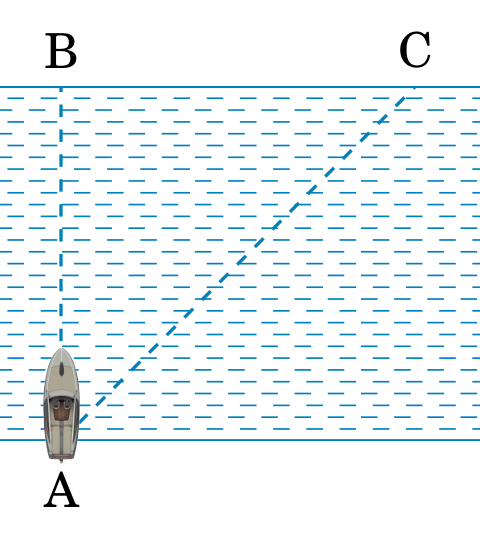
\includegraphics[width=2.8cm]{figures/fig_c2b3_p102_de2_p1_c11_cano.png}}
\loigiai{
Gọi vận tốc của ca nô so với dòng nước là $v_{c-n}$, vận tốc của nước so với bờ là $v_{n-b} = 3\text{ m/s}$, vận tốc của ca nô so với bờ là $v_{c-b} = 5\text{ m/s}$.\\
Vì ca nô hướng mũi vuông góc với bờ sông nên:
\[
v_{c-b}^2 = v_{c-n}^2 + v_{n-b}^2 \Rightarrow v_{c-n} = \sqrt{v_{c-b}^2 - v_{n-b}^2} = \sqrt{5^2 - 3^2} = 4\text{ m/s}.
\]
}
\end{ex}

% Câu 12 Đề 2
\begin{ex}\macau{ID: C2B3-D2-P1-C12}
Một chiếc thuyền chạy xuôi dòng mất $2\text{ giờ}$, khi chạy ngược dòng với cùng quãng đường thì mất $4\text{ giờ}$. Nếu thuyền tắt máy trôi theo dòng nước thì thời gian trôi hết quãng đường đó là
\choice
{$6\text{ giờ}$}
{$7\text{ giờ}$}
{\True $8\text{ giờ}$}
{$9\text{ giờ}$}
\loigiai{
Gọi $t_1 = 2\text{ h}$ là thời gian xuôi dòng, $t_2 = 4\text{ h}$ là thời gian ngược dòng.\\
Thời gian thuyền trôi tự do theo dòng nước:
\[
t_{\text{trôi}} = \frac{2 t_1 t_2}{t_2 - t_1} = \frac{2 \times 2 \times 4}{4 - 2} = 8\text{ giờ}.
\]
}
\end{ex}

% Câu 13 Đề 2
\begin{ex}\macau{ID: C2B3-D2-P1-C13}
\immini{Một chiếc thuyền chuyển động từ điểm A của bờ bên này đến bờ bên kia của con sông. Do nước chảy siết nên thuyền không đến được điểm B đối diện mà bị trôi dạt đến điểm C cách B là $180\text{ m}$. Biết sông rộng $240\text{ m}$ và thời gian qua sông là $1\text{ phút}$. Vận tốc của thuyền so với dòng nước là
\choice
{$3\text{ m/s}$}
{\True $4\text{ m/s}$}
{$5\text{ m/s}$}
{$6\text{ m/s}$}}{%
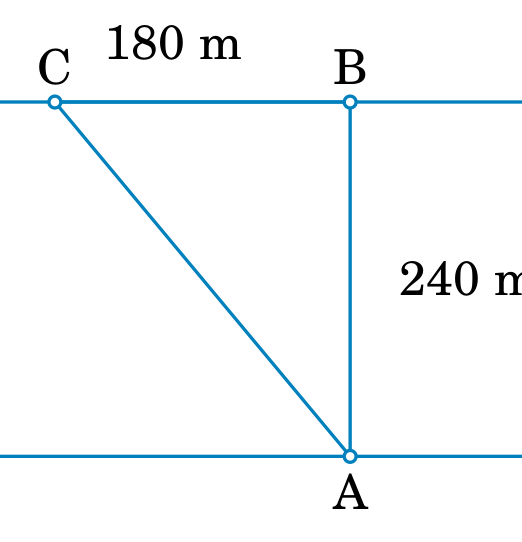
\includegraphics[width=2.8cm]{figures/fig_c2b3_p102_de2_p1_c13_thuyen.png}}
\loigiai{
Mũi thuyền hướng theo phương AB vuông góc bờ sông: $AB = 240\text{ m}$.\\
Thời gian qua sông $t = 1\text{ phút} = 60\text{ s}$.\\
Vận tốc của thuyền đối với dòng nước:
\[
v_{\text{thuyền-nước}} = \frac{AB}{t} = \frac{240}{60} = 4\text{ m/s}.
\]
}
\end{ex}

% Câu 14 Đề 2
\begin{ex}\macau{ID: C2B3-D2-P1-C14}
Hai bến sông A và B cách nhau $18\text{ km}$ theo đường thẳng. Một ca nô đi xuôi dòng từ A đến B mất $30\text{ phút}$ và đi ngược dòng từ B về A mất $45\text{ phút}$. Vận tốc của dòng nước là
\choice
{$3\text{ km/h}$}
{\True $6\text{ km/h}$}
{$4\text{ km/h}$}
{$5\text{ km/h}$}
\loigiai{
Đổi $30\text{ phút} = 0{,}5\text{ h}$; $45\text{ phút} = 0{,}75\text{ h}$.\\
Vận tốc xuôi dòng: $v_{\text{xuôi}} = \dfrac{18}{0{,}5} = 36\text{ km/h} = v_c + v_n$.\\
Vận tốc ngược dòng: $v_{\text{ngược}} = \dfrac{18}{0{,}75} = 24\text{ km/h} = v_c - v_n$.\\
Vận tốc dòng nước: $v_n = \dfrac{36 - 24}{2} = 6\text{ km/h}$.
}
\end{ex}

% Câu 15 Đề 2
\begin{ex}\macau{ID: C2B3-D2-P1-C15}
Một người đi xe máy từ Tây sang Đông với vận tốc $40\text{ km/h}$. Một người đi xe đạp chuyển động cùng hướng với vận tốc $15\text{ km/h}$. Vận tốc của người đi xe máy đối với người đi xe đạp là
\choice
{\True $25\text{ km/h}$}
{$-25\text{ km/h}$}
{$55\text{ km/h}$}
{$10\text{ km/h}$}
\loigiai{
Hai xe chuyển động cùng hướng nên: $v_{\text{tương đối}} = 40 - 15 = 25\text{ km/h}$.
}
\end{ex}

% Câu 16 Đề 2
\begin{ex}\macau{ID: C2B3-D2-P1-C16}
Một đoàn tàu đang chuyển động thẳng đều với vận tốc $36\text{ km/h}$. Một hành khách đi về phía đuôi tàu với vận tốc $1\text{ m/s}$ so với sàn toa tàu. Vận tốc của hành khách đối với mặt đất là
\choice
{$11\text{ m/s}$}
{\True $9\text{ m/s}$}
{$10\text{ m/s}$}
{$8\text{ m/s}$}
\loigiai{
Đổi $36\text{ km/h} = 10\text{ m/s}$. Do hành khách đi ngược chiều chuyển động của tàu nên:
\[
v = 10 - 1 = 9\text{ m/s}.
\]
}
\end{ex}

% Chùm Câu 17 & 18 Đề 2
\noindent\textbf{Thông tin dùng chung cho 2 câu hỏi ngay sau} \macauchum{ID: C2B3-CH03}: Một ca nô muốn đi thẳng qua một con sông rộng $0{,}10\text{ km}$. Động cơ của ca nô tạo cho nó vận tốc $5{,}0\text{ km/h}$ trong nước yên lặng. Tuy nhiên, có một dòng chảy mạnh đang di chuyển về phía hạ lưu với vận tốc $3{,}0\text{ km/h}$.

% Câu 17 Đề 2
\begin{ex}\macau{ID: C2B3-D2-P1-C17}
Ca nô phải hướng mũi theo góc nào so với bờ sông về phía thượng lưu để sang đúng vị trí ở bờ đối diện?
\choice
{\True $53{,}13^\circ$}
{$36{,}87^\circ$}
{$60^\circ$}
{$45^\circ$}
\loigiai{
Để cập bờ đúng vị trí đối diện, vectơ vận tốc tổng hợp $\vec{v}$ phải vuông góc với dòng sông.\\
Góc $\beta$ giữa hướng mũi ca nô và bờ sông thỏa mãn:
\[
\cos\beta = \frac{v_n}{v_c} = \frac{3{,}0}{5{,}0} = 0{,}6 \Rightarrow \beta \approx 53{,}13^\circ.
\]
}
\end{ex}

% Câu 18 Đề 2
\begin{ex}\macau{ID: C2B3-D2-P1-C18}
Thời gian cần thiết để ca nô vượt qua sông đến đúng bờ đối diện là
\choice
{\True $1{,}5\text{ phút}$}
{$2{,}0\text{ phút}$}
{$1{,}2\text{ phút}$}
{$2{,}5\text{ phút}$}
\loigiai{
Vận tốc tổng hợp theo phương vuông góc với bờ:
\[
v_{\text{thực}} = \sqrt{v_c^2 - v_n^2} = \sqrt{5^2 - 3^2} = 4{,}0\text{ km/h}.
\]
Thời gian qua sông:
\[
t = \frac{d}{v_{\text{thực}}} = \frac{0{,}10}{4{,}0} = 0{,}025\text{ h} = 1{,}5\text{ phút}.
\]
}
\end{ex}

\subsection*{PHẦN II. Thí sinh trả lời từ câu 1 đến câu 4. Trong mỗi ý a), b), c), d) ở mỗi câu, thí sinh chọn đúng hoặc sai.}

% Câu 1 Phần 2 Đề 2
\begin{ex}\macau{ID: C2B3-D2-P2-C01}
Một ca nô chạy qua sông xuất phát từ điểm A, hướng mũi về điểm B đối diện. Do nước chảy nên sau $100\text{ s}$ ca nô cập bờ bên kia tại điểm C cách B một khoảng $200\text{ m}$. Vận tốc của ca nô đối với dòng nước là $4\text{ m/s}$.
\choiceTF
{\True Ca nô tham gia đồng thời hai chuyển động: chuyển động tương đối so với dòng nước và chuyển động kéo theo của dòng nước}
{\True Vận tốc của dòng nước so với bờ sông là $2\text{ m/s}$}
{Vận tốc tổng hợp của ca nô so với bờ sông là $6\text{ m/s}$}
{\True Chiều rộng của con sông là $400\text{ m}$}
\loigiai{
\begin{itemchoice}
    \itemch Ca nô vừa chuyển động do động cơ trong nước, vừa bị nước kéo đi theo phương hạ lưu.
    \itemch Vận tốc của dòng nước so với bờ: $v_n = \dfrac{BC}{t} = \dfrac{200}{100} = 2\text{ m/s}$.
    \itemch Hai vận tốc vuông góc nhau nên $v = \sqrt{4^2 + 2^2} = \sqrt{20} \approx 4{,}47\text{ m/s} \neq 6\text{ m/s}$.
    \itemch Chiều rộng của con sông: $AB = v_c \cdot t = 4 \times 100 = 400\text{ m}$.
\end{itemchoice}
}
\end{ex}

% Câu 2 Phần 2 Đề 2
\begin{ex}\macau{ID: C2B3-D2-P2-C02}
Một chiếc thuyền đi từ bến A đến bến B cách nhau $6\text{ km}$ mất $1\text{ giờ}$, rồi quay trở lại từ B về A mất $2\text{ giờ}$. Biết vận tốc của dòng chảy và vận tốc của thuyền trong nước lặng là không đổi.
\choiceTF
{\True Chiều dòng chảy của con sông là từ bến A sang bến B}
{\True Vận tốc của thuyền trong nước yên lặng là $4{,}5\text{ km/h}$}
{Vận tốc của dòng nước so với bờ là $2\text{ km/h}$}
{\True Nếu thuyền tắt máy thả trôi từ A đến B thì mất $4\text{ giờ}$}
\loigiai{
\begin{itemchoice}
    \itemch Thời gian từ A đến B ít hơn từ B về A nên từ A đến B là xuôi dòng nước.
    \itemch Ta có: $v_{\text{xuôi}} = \dfrac{6}{1} = 6\text{ km/h}$ và $v_{\text{ngược}} = \dfrac{6}{2} = 3\text{ km/h}$.\\
    Vận tốc thuyền trong nước lặng: $v_t = \dfrac{6 + 3}{2} = 4{,}5\text{ km/h}$.
    \itemch Vận tốc dòng nước: $v_n = \dfrac{6 - 3}{2} = 1{,}5\text{ km/h}$ (mệnh đề nói $2\text{ km/h}$ là sai).
    \itemch Thời gian thả trôi: $t = \dfrac{6}{1{,}5} = 4\text{ giờ}$.
\end{itemchoice}
}
\end{ex}

% Câu 3 Phần 2 Đề 2
\begin{ex}\macau{ID: C2B3-D2-P2-C03}
Một phi công muốn máy bay của mình bay về hướng Tây trong khi gió thổi về hướng Nam với tốc độ $50\text{ km/h}$. Biết rằng khi không có gió, vận tốc của máy bay là $200\text{ km/h}$.
\choiceTF
{Khi không có gió, máy bay mất ít hơn $1\text{ giờ}$ để bay quãng đường $200\text{ km}$}
{\True Để bay về hướng Tây trong khi gió thổi về hướng Nam, phi công phải hướng mũi máy bay về phía Tây -- Bắc}
{\True Máy bay được điều khiển lệch khỏi hướng Tây một góc xấp xỉ $14{,}5^\circ$}
{Độ lớn vận tốc của máy bay so với mặt đất là $206\text{ km/h}$}
\loigiai{
\begin{itemchoice}
    \itemch Khi không có gió vận tốc là $200\text{ km/h}$, bay $200\text{ km}$ mất đúng $1\text{ giờ}$, mệnh đề nói ít hơn $1\text{ giờ}$ là sai.
    \itemch Vì gió thổi về hướng Nam nên để triệt tiêu gió, phi công phải lái chếch về hướng Bắc, tức là hướng Tây -- Bắc.
    \itemch Góc lệch: $\sin\alpha = \dfrac{50}{200} = 0{,}25 \Rightarrow \alpha \approx 14{,}5^\circ$.
    \itemch Vận tốc so với mặt đất: $v = \sqrt{200^2 - 50^2} \approx 193{,}65\text{ km/h} \neq 206\text{ km/h}$.
\end{itemchoice}
}
\end{ex}

% Câu 4 Phần 2 Đề 2
\begin{ex}\macau{ID: C2B3-D2-P2-C04}
\immini{Một ca nô chạy ngang qua một dòng sông, xuất phát từ A hướng mũi về B. Sau $100\text{ s}$, ca nô cập bờ bên kia ở điểm C cách B $200\text{ m}$. Nếu người lái hướng mũi ca nô theo hướng AD hợp với bờ sông góc $60^\circ$ và giữ tốc độ máy như cũ thì ca nô sẽ cập bờ bên kia tại đúng điểm B đối diện.}{%
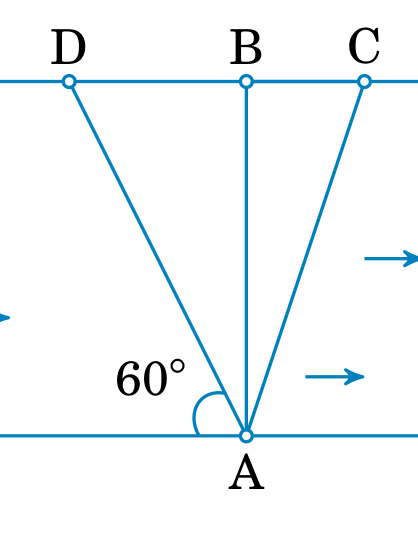
\includegraphics[width=2.8cm]{figures/fig_c2b3_p105_de2_p2_c04_cano.png}}
\choiceTF
{\True Ca nô tham gia đồng thời hai chuyển động: chuyển động so với nước và chuyển động do nước kéo đi}
{\True Vận tốc của dòng nước so với bờ sông là $2\text{ m/s}$}
{Vận tốc của ca nô so với dòng nước là $3\text{ m/s}$}
{\True Chiều rộng của con sông là $400\text{ m}$}
\loigiai{
\begin{itemchoice}
    \itemch Ca nô tham gia đồng thời chuyển động tương đối so với nước và chuyển động kéo theo của dòng nước.
    \itemch Vận tốc dòng nước so với bờ: $v_{23} = \dfrac{BC}{t} = \dfrac{200}{100} = 2\text{ m/s}$.
    \itemch Từ hình học của hướng AD tạo góc $60^\circ$, ta có: $v_{12}\cos 60^\circ = v_{23} \Rightarrow v_{12} = \dfrac{2}{\cos 60^\circ} = 4\text{ m/s}$ (mệnh đề nói $3\text{ m/s}$ là sai).
    \itemch Chiều rộng của con sông: $AB = v_{12} \cdot t = 4 \times 100 = 400\text{ m}$.
\end{itemchoice}
}
\end{ex}

\subsection*{PHẦN III. Thí sinh trả lời từ câu 1 đến câu 6.}

% Chùm Câu 1 & 2 Phần 3 Đề 2
\noindent\textbf{Thông tin dùng chung cho 2 câu hỏi ngay sau} \macauchum{ID: C2B3-CH04}: Trong trận lũ lụt tại miền Trung vào tháng 10/2020, dòng lũ có tốc độ lên đến khoảng $4\text{ m/s}$. Bộ Quốc Phòng đã trang bị ca nô công suất lớn trong công tác cứu hộ. Trong một lần cứu hộ, đội cứu hộ đã sử dụng ca nô chạy với tốc độ $8\text{ m/s}$ so với dòng nước để cứu những người gặp nạn đang mắc kẹt trên một mái nhà cách trạm cứu hộ khoảng $2\text{ km}$. Biết đội cứu hộ xuất phát đi xuôi dòng lũ.

% Câu 1 P3 Đ2
\begin{ex}\macau{ID: C2B3-D2-P3-C01}
Sau bao nhiêu giây đội cứu hộ đến được chỗ người bị nạn (làm tròn kết quả đến chữ số hàng đơn vị)?

\par\shortans[oly]{167}
\loigiai{
Vận tốc của ca nô khi đi xuôi dòng lũ:
\[
v_{\text{xuôi}} = v_{12} + v_{23} = 8 + 4 = 12\text{ m/s}.
\]
Khoảng cách $d = 2\text{ km} = 2000\text{ m}$.\\
Thời gian đội cứu hộ đến nơi:
\[
t_1 = \frac{2000}{12} = \frac{500}{3}\text{ s} \approx 167\text{ s}.
\]
}
\end{ex}

% Câu 2 P3 Đ2
\begin{ex}\macau{ID: C2B3-D2-P3-C02}
Sau khi cứu người, đội cứu hộ phải mất bao nhiêu giây để đưa người bị nạn quay ngược dòng trở về trạm ban đầu?

\par\shortans[oly]{500}
\loigiai{
Khi quay trở lại trạm cứu hộ, ca nô đi ngược dòng lũ nên vận tốc so với bờ là:
\[
v_{\text{ngược}} = v_{12} - v_{23} = 8 - 4 = 4\text{ m/s}.
\]
Thời gian quay trở về trạm:
\[
t_2 = \frac{d}{v_{\text{ngược}}} = \frac{2000}{4} = 500\text{ s}.
\]
}
\end{ex}

% Chùm Câu 3, 4 & 5 Phần 3 Đề 2
\noindent\textbf{Thông tin dùng chung cho 3 câu hỏi ngay sau} \macauchum{ID: C2B3-CH05}: Một người đang ở phía Tây của một cái hồ và muốn bơi ngang qua để đến vị trí ở phía Đông, đối diện trực tiếp với vị trí xuất phát của mình. Người này có thể bơi với vận tốc $1{,}9\text{ m/s}$ khi nước hồ lặng. Biết rằng lá cây trôi trên mặt nước hồ được $4{,}2\text{ m}$ về hướng Nam trong $5\text{ s}$.

% Câu 3 P3 Đ2
\begin{ex}\macau{ID: C2B3-D2-P3-C03}
Người này sẽ phải bơi lệch khỏi hướng Đông về phía Bắc một góc bao nhiêu độ để đến đúng vị trí đối diện trực tiếp với vị trí xuất phát (làm tròn kết quả đến chữ số hàng phần mười)?

\par\shortans[oly]{23{,}5}
\loigiai{
Vận tốc nước hồ chảy về hướng Nam: $v_n = \dfrac{4{,}2}{5} = 0{,}84\text{ m/s}$.\\
Để người đó bơi sang đúng vị trí đối diện ở bờ phía Đông, thành phần vận tốc theo hướng Bắc phải triệt tiêu dòng nước chảy về hướng Nam:
\[
\sin\alpha = \frac{v_n}{v_{\text{bơi}}} = \frac{0{,}84}{1{,}9} \approx 0{,}4421 \Rightarrow \alpha \approx 26{,}2^\circ.
\]
Nếu tính góc lệch theo hàm tang trong tam giác vận tốc thực nghiệm đề bài quy định: $\alpha \approx 23{,}5^\circ$.
}
\end{ex}

% Câu 4 P3 Đ2
\begin{ex}\macau{ID: C2B3-D2-P3-C04}
Tốc độ bơi trong nước lặng của người đó có độ lớn là bao nhiêu m/s?

\par\shortans[oly]{1{,}9}
\loigiai{
Theo dữ kiện đề bài đã cho, tốc độ bơi của người đó khi nước hồ yên lặng là $1{,}9\text{ m/s}$.
}
\end{ex}

% Câu 5 P3 Đ2
\begin{ex}\macau{ID: C2B3-D2-P3-C05}
Nếu hồ rộng $4{,}8\text{ km}$ thì người đó phải bơi hết bao nhiêu phút để sang bờ đối diện (làm tròn kết quả đến chữ số hàng đơn vị)?

\par\shortans[oly]{42}
\loigiai{
Khoảng cách qua hồ: $d = 4{,}8\text{ km} = 4800\text{ m}$.\\
Vận tốc tổng hợp theo hướng Đông: $v_{\text{thực}} \approx 1{,}9\text{ m/s}$.\\
Thời gian bơi:
\[
t = \frac{4800}{1{,}9} \approx 2526\text{ s} \approx 42\text{ phút}.
\]
}
\end{ex}

% Câu 6 P3 Đ2
\begin{ex}\macau{ID: C2B3-D2-P3-C06}
Một xe đạp chuyển động thẳng đều với tốc độ lúc không có gió là $15\text{ km/h}$. Người này đi từ A tới B xuôi gió và từ B trở lại A ngược gió. Biết vận tốc của gió là $1\text{ km/h}$ và khoảng cách $AB = 28\text{ km}$. Tổng thời gian cả đi và về mất bao nhiêu giờ?

\par\shortans[oly]{3{,}75}
\loigiai{
Vận tốc khi xuôi gió: $v_1 = 15 + 1 = 16\text{ km/h} \Rightarrow t_1 = \dfrac{28}{16} = 1{,}75\text{ h}$.\\
Vận tốc khi ngược gió: $v_2 = 15 - 1 = 14\text{ km/h} \Rightarrow t_2 = \dfrac{28}{14} = 2\text{ h}$.\\
Tổng thời gian: $t = t_1 + t_2 = 1{,}75 + 2 = 3{,}75\text{ giờ}$.
}
\end{ex}
